%Version 3.1 December 2024
% See section 11 of the User Manual for version history
%
%%%%%%%%%%%%%%%%%%%%%%%%%%%%%%%%%%%%%%%%%%%%%%%%%%%%%%%%%%%%%%%%%%%%%%
%%                                                                 %%
%% Please do not use \input{...} to include other tex files.       %%
%% Submit your LaTeX manuscript as one .tex document.              %%
%%                                                                 %%
%% All additional figures and files should be attached             %%
%% separately and not embedded in the \TeX\ document itself.       %%
%%                                                                 %%
%%%%%%%%%%%%%%%%%%%%%%%%%%%%%%%%%%%%%%%%%%%%%%%%%%%%%%%%%%%%%%%%%%%%%

%%\documentclass[referee,sn-basic]{sn-jnl}% referee option is meant for double line spacing

%%=======================================================%%
%% to print line numbers in the margin use lineno option %%
%%=======================================================%%

%%\documentclass[lineno,pdflatex,sn-basic]{sn-jnl}% Basic Springer Nature Reference Style/Chemistry Reference Style

%%=========================================================================================%%
%% the documentclass is set to pdflatex as default. You can delete it if not appropriate.  %%
%%=========================================================================================%%

%%\documentclass[sn-basic]{sn-jnl}% Basic Springer Nature Reference Style/Chemistry Reference Style

%%Note: the following reference styles support Namedate and Numbered referencing. By default the style follows the most common style. To switch between the options you can add or remove “Numbered” in the optional parenthesis. 
%%The option is available for: sn-basic.bst, sn-chicago.bst%  
 
%%\documentclass[pdflatex,sn-nature]{sn-jnl}% Style for submissions to Nature Portfolio journals
%%\documentclass[pdflatex,sn-basic]{sn-jnl}% Basic Springer Nature Reference Style/Chemistry Reference Style
%%\documentclass[pdflatex,sn-mathphys-num]{sn-jnl}% Math and Physical Sciences Numbered Reference Style
%%\documentclass[pdflatex,sn-mathphys-ay]{sn-jnl}% Math and Physical Sciences Author Year Reference Style
%%\documentclass[pdflatex,sn-aps]{sn-jnl}% American Physical Society (APS) Reference Style
%%\documentclass[pdflatex,sn-vancouver-num]{sn-jnl}% Vancouver Numbered Reference Style
%%\documentclass[pdflatex,sn-vancouver-ay]{sn-jnl}% Vancouver Author Year Reference Style
%%\documentclass[pdflatex,sn-apa]{sn-jnl}% APA Reference Style
%%\documentclass[pdflatex,sn-chicago]{sn-jnl}% Chicago-based Humanities Reference Style

%%%% Standard Packages
%%<additional latex packages if required can be included here>

%%\documentclass[pdflatex,sn-mathphys-num]{sn-jnl}

\documentclass[referee,lineno,pdflatex,sn-mathphys-ay]{sn-jnl}


\usepackage{graphicx}%
\usepackage{multirow}%
\usepackage{amsmath,amssymb,amsfonts}%
\usepackage{mathrsfs}%
\usepackage{xcolor}%
\usepackage{textcomp}%
\usepackage{manyfoot}%
\usepackage{booktabs}%
\usepackage{algorithm}%
\usepackage{algorithmicx}%
\usepackage{algpseudocode}%
\usepackage{listings}%
\usepackage{array}%
\usepackage{url}

\newcommand{\orcidtext}[1]{\href{https://orcid.org/#1}{\textsuperscript{[ORCID]}}}

%%%%

%%%%%=============================================================================%%%%
%%%%  Remarks: This template is provided to aid authors with the preparation
%%%%  of original research articles intended for submission to journals published 
%%%%  by Springer Nature. The guidance has been prepared in partnership with 
%%%%  production teams to conform to Springer Nature technical requirements. 
%%%%  Editorial and presentation requirements differ among journal portfolios and 
%%%%  research disciplines. You may find sections in this template are irrelevant 
%%%%  to your work and are empowered to omit any such section if allowed by the 
%%%%  journal you intend to submit to. The submission guidelines and policies 
%%%%  of the journal take precedence. A detailed User Manual is available in the 
%%%%  template package for technical guidance.
%%%%%=============================================================================%%%%

%% as per the requirement new theorem styles can be included as shown below
\theoremstyle{thmstyleone}%
\newtheorem{theorem}{Theorem}%  meant for continuous numbers
%%\newtheorem{theorem}{Theorem}[section]% meant for sectionwise numbers
%% optional argument [theorem] produces theorem numbering sequence instead of independent numbers for Proposition
\newtheorem{proposition}[theorem]{Proposition}% 
%%\newtheorem{proposition}{Proposition}% to get separate numbers for theorem and proposition etc.

\theoremstyle{thmstyletwo}%
\newtheorem{example}{Example}%
\newtheorem{remark}{Remark}%

\theoremstyle{thmstylethree}%
\newtheorem{definition}{Definition}%

\raggedbottom
%%\unnumbered% uncomment this for unnumbered level heads

\begin{document}

\title[Quantum Kernels under Distribution Shift]{Evaluation Choices Determine Apparent Quantum-Kernel Robustness under Distribution Shift}


%%=============================================================%%
%% GivenName	-> \fnm{Joergen W.}
%% Particle	-> \spfx{van der} -> surname prefix
%% FamilyName	-> \sur{Ploeg}
%% Suffix	-> \sfx{IV}
%% \author*[1,2]{\fnm{Joergen W.} \spfx{van der} \sur{Ploeg} 
%%  \sfx{IV}}\email{iauthor@gmail.com}
%%=============================================================%%



\author*[1]{\fnm{Roberto} \sur{Fernández-Barrios}\orcidtext{0009-0003-5312-2634}}\email{roberto.fernandez.b@deusto.es}

\author[1]{\fnm{Iker} \sur{Pastor-López}\orcidtext{0000-0002-3068-6248}}\email{iker.pastor@deusto.es}

\author[1]{\fnm{Asier} \sur{González-Santocildes}\orcidtext{0009-0002-8888-8560}}\email{gonzalez.asier@deusto.es}

\author[1]{\fnm{Pablo} \sur{García Bringas}\orcidtext{0000-0003-3594-9534}}\email{pablo.garcia.bringas@deusto.es}

\affil*[1]{\orgdiv{Faculty of Engineering}, \orgname{University of Deusto}, \orgaddress{\street{Avda. de las Universidades, 24.}, \city{Bilbao}, \postcode{48007}, \country{Spain}}}

%%==================================%%
%% Sample for unstructured abstract %%
%%==================================%%

\abstract{Quantum-kernel robustness claims depend on how candidates are tuned and selected. We test this dependence in a controlled kernel-swap benchmark spanning four security scenarios, three shift mechanisms, two classifiers and fifteen pipeline realizations per setting. Under same-test OOD-oracle selection and fixed regularization, fidelity kernels appear to improve balanced accuracy over linear and radial-basis-function baselines by up to $+0.037$. When regularization is tuned from training data, selection uses no OOD labels and candidate budgets are matched, the dataset-equal quantum-minus-classical effect becomes $-0.005$ for support-vector classification and $-0.002$ for Gaussian-process classification. The primary support-vector result is classical-favoured or conditionally tied in seven of eight scenario-groups. At matched effective rank, classical kernels are at least as accurate in every group. Effective rank and OOD kernel-target alignment are associated with accuracy but favour neither family, while finite-shot estimation distorts exact-statevector effective rank. Evaluation therefore removes the apparent robustness advantage within the low-qubit regimes studied.}



%%================================%%
%% Sample for structured abstract %%
%%================================%%

% \abstract{\textbf{Purpose:} The abstract serves both as a general introduction to the topic and as a brief, non-technical summary of the main results and their implications. The abstract must not include subheadings (unless expressly permitted in the journal's Instructions to Authors), equations or citations. As a guide the abstract should not exceed 200 words. Most journals do not set a hard limit however authors are advised to check the author instructions for the journal they are submitting to.
% 
% \textbf{Methods:} The abstract serves both as a general introduction to the topic and as a brief, non-technical summary of the main results and their implications. The abstract must not include subheadings (unless expressly permitted in the journal's Instructions to Authors), equations or citations. As a guide the abstract should not exceed 200 words. Most journals do not set a hard limit however authors are advised to check the author instructions for the journal they are submitting to.
% 
% \textbf{Results:} The abstract serves both as a general introduction to the topic and as a brief, non-technical summary of the main results and their implications. The abstract must not include subheadings (unless expressly permitted in the journal's Instructions to Authors), equations or citations. As a guide the abstract should not exceed 200 words. Most journals do not set a hard limit however authors are advised to check the author instructions for the journal they are submitting to.
% 
% \textbf{Conclusion:} The abstract serves both as a general introduction to the topic and as a brief, non-technical summary of the main results and their implications. The abstract must not include subheadings (unless expressly permitted in the journal's Instructions to Authors), equations or citations. As a guide the abstract should not exceed 200 words. Most journals do not set a hard limit however authors are advised to check the author instructions for the journal they are submitting to.}

\keywords{quantum machine learning; quantum kernels; distribution shift; out-of-distribution robustness; kernel methods; kernel-target alignment; Gaussian processes; malware detection; network intrusion detection}

%%\pacs[JEL Classification]{D8, H51}

%%\pacs[MSC Classification]{35A01, 65L10, 65L12, 65L20, 65L70}

\maketitle

\section{Introduction}
\label{sec:introduction}

Quantum kernel methods embed classical data into quantum states and use state overlaps as similarities for otherwise classical learners \cite{havlicek2019quantumenhanced,schuld2019featurehilbert,schuld2021kernelmethods}. This separation makes them a clean setting for asking whether quantum-induced feature geometry provides useful inductive bias. It also makes comparison unusually sensitive to evaluation design: the downstream learner can be held fixed, but conclusions still depend on the encoding, bandwidth, regularization, classical reference set, and rule used to select a candidate \cite{huang2021powerofdata,schuld2021encoding,bowles2024betterthanclassical,schnabel2025scrutiny}.

Recent benchmarks have accordingly shifted the question from whether an isolated quantum model can perform well to whether a claimed gain survives strong and symmetric controls. Broad QML studies find competitive classical baselines once pipelines are aligned \cite{bowles2024betterthanclassical}; quantum-kernel benchmarks show substantial sensitivity to feature map and hyperparameter choice \cite{schnabel2025scrutiny}; and a concurrent tabular study using nested cross-validation, spectral analysis, and hardware validation finds no significant quantum win across its tested pairs \cite{kakavand2026benchmarking}. These studies evaluate predominantly identically distributed train--test settings. They do not address a further deployment question: what happens when the target distribution changes and its labels cannot be used to choose the deployed kernel?

Distribution shift makes model selection part of the estimand. Work on domain generalization and real-world shift has shown that robustness gains can disappear when search budgets, hyperparameters, and selection criteria are standardized \cite{gulrajani2021domainbed,koh2021wilds,yao2022wildtime,zhou2023dgsurvey}. A selector that inspects the shifted test labels estimates an oracle upper bound, not deployable performance; a family with more candidates has more opportunities to win that selection. Fair quantum--classical evaluation under shift must therefore control not only the classifier and data split, but also regularization, candidate budget, and label access.

Security detection provides a useful stress test because shift is intrinsic to the application. Malware evolves over time, and experimental bias can overstate detector performance \cite{anderson2018ember,pendlebury2019tesseract,arp2022dosdonts}; network traffic changes with infrastructure and attack campaigns \cite{moustafa2015unsw,alsaedi2020toniot}. Quantum classifiers have already been evaluated on intrusion-detection benchmarks, sometimes with reported gains over small classical reference sets on i.i.d.\ splits \cite{abreu2024qmlids,abreu2025quantumnetsec,bellante2025evaluating}. We use these datasets not to propose a security system, but to expose kernel families to reproducible constructed shifts and to a held-out attack-campaign shift.

The closest robustness-specific concurrent work studies additive input corruption and proposes a spectral phase encoding \cite{herrero2026spectralphase}. Our question is complementary: rather than optimize a new encoding, we audit how evaluation choices change a family-level conclusion under constructed and held-out-campaign shifts. The distinguishing axes are no-OOD-label selection, equal candidate budgets, per-configuration train-only regularization, fixed-case inference, and a geometry analysis tied specifically to behaviour after the distribution moves.

We implement a controlled \emph{kernel-swap} benchmark in which preprocessing, splits, classifier, and family-internal selection logic are fixed while only the kernel changes. Four security scenarios from EMBER, UNSW-NB15, and ToN-IoT yield eight scenario-groups across constructed and held-out-campaign shifts. Support-vector and Laplace Gaussian-process classifiers consume the same precomputed Gram matrices. The quantum family contains four fidelity feature-map families with angle-scale sweeps; the classical family extends linear and RBF references with polynomial, Laplacian, and Mat\'ern kernels and symmetric bandwidth freedom. Each configuration's regularization is tuned from training data alone. The primary deployed candidate is selected on a disjoint ID-validation split, and the two extended families receive equal candidate budgets. Fifteen pipeline realizations per setting quantify conditional variability; the benchmarks are treated as fixed case studies rather than as random draws from an undefined population.

The comparison is coupled to a mechanistic audit. We measure effective rank, centered kernel-target alignment, concentration, and geometric difference \cite{roy2007effective,cristianini2001kta,cortes2012centeredalignment,huang2021powerofdata}; use partial association, leave-one-dataset-out prediction, and effective-rank matching to restrict interpretation; and perturb fidelity estimates with finite shots to test whether exact statevector geometry survives measurement.

The evaluation choices change the conclusion. With same-test oracle selection, fixed regularization, and customary linear+RBF baselines, fidelity kernels appear to improve OOD balanced accuracy by as much as $+0.037$. With train-only regularization, no-OOD-label selection, and equal candidate budgets, the dataset-equal quantum-minus-classical delta is $-0.005$ for SVC and $-0.002$ for the GP classifier. The primary SVC comparison is classical-favoured or conditionally tied in seven of eight scenario-groups. Effective rank and OOD alignment remain associated with accuracy, but the association is regime-dependent and shared by both families; at matched effective rank, the classical configuration is at least as accurate in every group. Finite-shot estimation inflates effective rank and destabilizes candidate selection.

The contribution is therefore an evaluation result rather than an advantage claim: it identifies which protocol choices create the optimistic quantum-kernel robustness result, supplies a deployable equal-budget comparison under shift, and shows that the observed geometry does not uniquely identify quantum provenance. The scope is deliberately limited to the low-qubit fidelity kernels, datasets, and shift constructions studied here.

% Figure generated by scripts/reporting/make_v4_figures.py
\begin{figure*}[t]
\centering
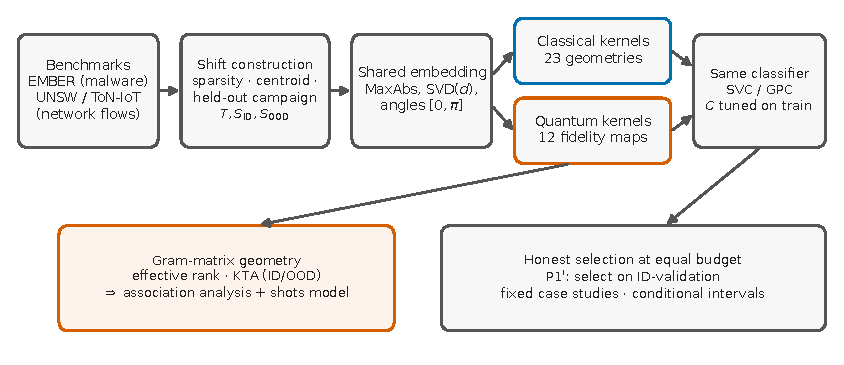
\includegraphics[width=\textwidth]{fig_v4_protocol.pdf}
\caption{The controlled kernel-swap protocol. Benchmark pools feed reproducible shift constructions; all kernels operate on a shared train-only embedding, receive per-configuration regularization tuned on the training split, and are consumed by the same precomputed-kernel classifiers. Family-level conclusions are drawn by honest, equal-budget selection on an in-distribution validation split (P1$'$), summarized as fixed case studies with conditional intervals; the Gram matrices feed the geometry-association analysis and the finite-shot model.}
\label{fig:protocol}
\end{figure*}

\section{Results}
\label{sec:results}

\subsection{Overview}

We report results under the controlled kernel-swap protocol described in Section~\ref{sec:methods}. All comparisons share the same classifier, preprocessing pipeline, and ID/OOD split definitions within a scenario-group; the only varying component is the kernel, and every number below aggregates fifteen pipeline realizations per setting. The argument proceeds in three movements. First, under test-peeking oracle selection and fixed regularization, the fidelity kernels show an apparent OOD advantage over linear and RBF baselines (Section~\ref{sec:res_baselines}). Second, we tune each configuration on training data alone, select on an in-distribution validation split disjoint from both test splits, and match the candidate budgets of the extended families. Under this controlled comparison no robust family-level advantage remains; the primary SVC comparison is classical-favoured or tied in seven of eight scenario-groups (Section~\ref{sec:res_honest}). Third, a geometry analysis shows that effective rank and OOD alignment are associated with---but do not causally determine---performance, that the association is regime-dependent, and that it favours neither family (Section~\ref{sec:res_mechanism}); a finite-shot analysis then shows the exact geometry does not transfer unchanged to finite measurement (Section~\ref{sec:res_shots}). Throughout, we treat the eight scenario-groups as fixed case studies and report effect sizes with conditional intervals rather than a population $p$-value, because the settings within a benchmark share data pools and are not exchangeable (Section~\ref{sec:methods}).

\subsection{The apparent advantage under oracle selection}
\label{sec:res_baselines}

We begin with the comparison that dominates the literature: fidelity-based quantum kernels against linear and RBF baselines, with each family's representative chosen by Best-by-OOD selection---the configuration with the highest balanced accuracy on the OOD test split itself---and the classical kernels left at the default regularization $C=1$. Under these conventions, on EMBER, the quantum family shows an OOD advantage of $+0.037$ under SVC and $+0.028$ under the GP classifier against linear+RBF, shrinking to $+0.004$/$+0.002$ once the classical family is enlarged with heavier-tailed kernels. Supplementary Table~2 gives the complete oracle results.

Two features favour this apparent quantum result. Best-by-OOD is an \emph{oracle}: it uses the labels it then reports. Fixing $C=1$ also leaves classical candidates at a potentially unsuitable regularization point. These values are therefore descriptive upper bounds, not deployable effects.

\subsection{A fair comparison removes the advantage}
\label{sec:res_honest}

A deployable comparison must tune each configuration's regularization without looking at the test data, select the deployed configuration without OOD labels, and compare families at the same candidate budget. We implement all three (Section~\ref{sec:methods}). For every kernel candidate, the SVC regularization $C$ is chosen by five-fold cross-validation on the training Gram matrix alone. The deployed configuration is then the one with the best balanced accuracy on an in-distribution \emph{validation} split, held out from the ID test split (protocol P1$'$); no OOD label is ever consulted in selection. The primary comparison uses the same candidate budget for both extended families (60 per family in full-coverage groups and 20 in reduced-coverage groups), with the full classical pool retained as a sensitivity. We treat the eight scenario-groups as fixed case studies and report, per group, the quantum-minus-classical OOD delta with a conditional interval over the five split realizations, and no population $p$-value (Section~\ref{sec:methods}).

Table~\ref{tab:headline} and Figure~\ref{fig:honest} give the result: no robust advantage remains against either reference. Against the equal-budget extended classical family, the P1$'$ delta is classical-favoured or within the conditional uncertainty of zero in seven of the eight scenario-groups under the primary SVC comparison, with a dataset-equal-weighted mean of $-0.005$ (leave-one-dataset-out range $[-0.006,-0.004]$); under the GP classifier the mean is $-0.002$ ($[-0.003,+0.000]$). Against the customary linear+RBF baseline---the comparison that produced the $+0.037$ oracle result of Section~\ref{sec:res_baselines}---the no-OOD-label delta is $-0.004$ under SVC and $+0.004$ under the GP classifier, with heterogeneous signs across scenario-groups. The single regime that retains a small quantum lean under both equal-budget comparisons is UNSW-NB15 reconnaissance under held-out attack-campaign shift ($+0.005$ for both classifiers); both conditional intervals include zero. The full-pool extended-family sensitivity is similar in direction and scale (dataset-equal means $-0.004$ for both classifiers), so the conclusion does not depend on giving the classical family its larger pool.

% Headline honest-selection table; rows from scripts/reporting/make_v4_tables.py
% (results/v4/tables/table_headline.tex)
\begin{table*}[t]
\centering
\caption{No-OOD-label selection results (eight scenario-groups, fifteen pipeline realizations per setting). Quantum-minus-classical OOD balanced-accuracy delta under P1$'$ (select on ID-validation, tune per-configuration $C$ on train, evaluate on OOD test). The extended-family comparison is the frozen equal-budget analysis: 60 candidates per family in full-coverage groups and 20 in reduced-coverage groups. Its interval is conditional pipeline-realization uncertainty over the five split seeds. The customary linear+RBF comparison is contextual rather than an equal-budget endpoint; the full-pool extended-family sensitivity remains in the machine-readable artifact. No population $p$-value is reported.}
\label{tab:headline}
\scriptsize
\setlength{\tabcolsep}{3pt}
\begin{tabular}{@{}llccc@{}}
\toprule
Scenario & Clf. & vs lin./RBF & vs ext. (equal $B$) & conditional interval \\
\midrule
\multirow{2}{*}{EMBER $m1$} & SVC & $-0.0095$ & $-0.0058$ & $[-0.0340, +0.0223]$ \\
 & GPC & $-0.0050$ & $-0.0009$ & $[-0.0101, +0.0083]$ \\
\addlinespace
\multirow{2}{*}{EMBER $m2$} & SVC & $+0.0139$ & $-0.0064$ & $[-0.0137, +0.0009]$ \\
 & GPC & $+0.0149$ & $+0.0027$ & $[-0.0027, +0.0081]$ \\
\addlinespace
\multirow{2}{*}{UNSW-DoS (campaign)} & SVC & $-0.0043$ & $-0.0033$ & $[-0.0139, +0.0073]$ \\
 & GPC & $+0.0041$ & $-0.0057$ & $[-0.0120, +0.0005]$ \\
\addlinespace
\multirow{2}{*}{UNSW-DoS (constructed)} & SVC & $-0.0085$ & $-0.0044$ & $[-0.0119, +0.0031]$ \\
 & GPC & $-0.0056$ & $-0.0108$ & $[-0.0177, -0.0039]$ \\
\addlinespace
\multirow{2}{*}{UNSW-Recon (campaign)} & SVC & $+0.0004$ & $+0.0050$ & $[-0.0058, +0.0157]$ \\
 & GPC & $+0.0074$ & $+0.0052$ & $[-0.0019, +0.0123]$ \\
\addlinespace
\multirow{2}{*}{UNSW-Recon (constructed)} & SVC & $-0.0076$ & $-0.0089$ & $[-0.0146, -0.0031]$ \\
 & GPC & $-0.0083$ & $-0.0075$ & $[-0.0208, +0.0059]$ \\
\addlinespace
\multirow{2}{*}{ToN-IoT (campaign)} & SVC & $-0.0172$ & $-0.0148$ & $[-0.0268, -0.0029]$ \\
 & GPC & $-0.0046$ & $-0.0090$ & $[-0.0190, +0.0010]$ \\
\addlinespace
\multirow{2}{*}{ToN-IoT (constructed)} & SVC & $-0.0016$ & $-0.0011$ & $[-0.0049, +0.0028]$ \\
 & GPC & $+0.0313$ & $+0.0109$ & $[+0.0017, +0.0202]$ \\
\midrule
\multicolumn{2}{@{}l}{Dataset-equal mean, SVC} & $-0.0043$ & $-0.0050$ & $[-0.0060, -0.0040]$ \\
\multicolumn{2}{@{}l}{Dataset-equal mean, GPC} & $+0.0043$ & $-0.0019$ & $[-0.0028, +0.0003]$ \\
\bottomrule
\end{tabular}
\end{table*}

% Figure generated by scripts/reporting/make_v4_figures.py
\begin{figure*}[t]
\centering
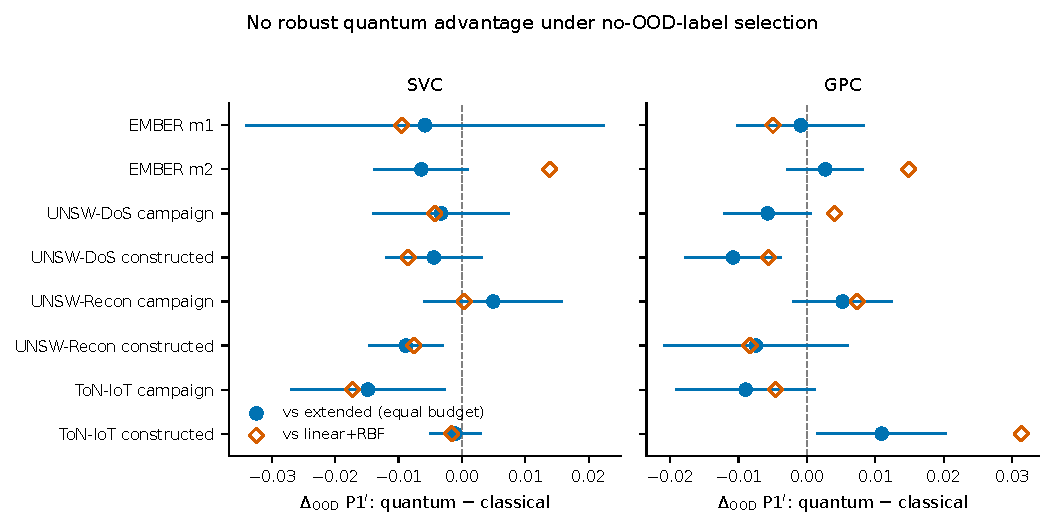
\includegraphics[width=\textwidth]{fig_v4_honest.pdf}
\caption{No robust quantum advantage under no-OOD-label selection. Per-scenario-group P1$'$ OOD deltas (quantum minus classical), for SVC (left) and the GP classifier (right). Filled circles compare against the equal-budget extended classical family with conditional pipeline-realization intervals; open diamonds compare against the customary linear+RBF reference. All eight scenario-groups are shown.}
\label{fig:honest}
\end{figure*}

\paragraph{Rank matching does not reveal a residual quantum advantage.} We pair each quantum configuration with the classical configuration of nearest training effective rank, within the same run and dimension, and compare their OOD accuracy. Figure~\ref{fig:rankmatched} reports the outcome: in all eight scenario-groups the median rank-matched delta is negative (quantum minus classical, between $-0.001$ and $-0.009$), and the quantum configuration is the more accurate of the pair in only 22--37\% of matches. Within the overlap covered by this observational matching, classical kernels are therefore at least as accurate at comparable effective rank.

% Figure generated by scripts/reporting/make_v4_figures.py
\begin{figure}[t]
\centering
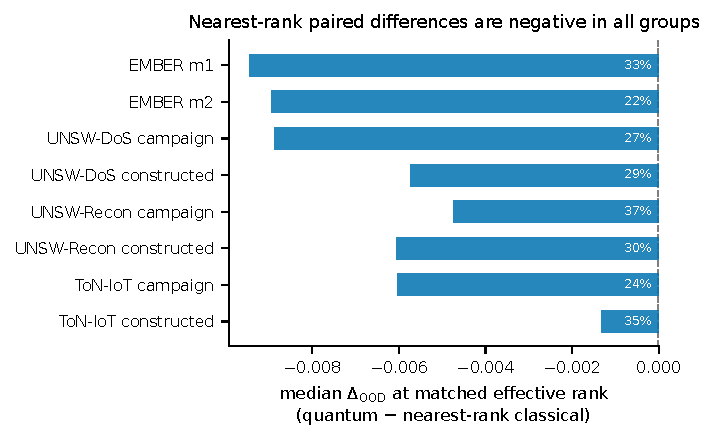
\includegraphics[width=\columnwidth]{fig_v4_rankmatched.pdf}
\caption{At matched effective rank, classical kernels are at least as accurate. For each quantum configuration we find the classical configuration of nearest training effective rank (within run and dimension) and take the OOD balanced-accuracy difference; bars are per-scenario-group medians, annotated with the fraction of matched pairs in which the quantum configuration is the more accurate.}
\label{fig:rankmatched}
\end{figure}

\subsection{Geometry is associated with, but does not determine, robustness}
\label{sec:res_mechanism}

The two families are close because both reach similar kernel geometry, and geometry---not quantumness---is what carries information about behaviour under shift. That information, however, is partial: it is a regime-dependent association, not the single governing law that optimistic accounts (our own earlier report included) proposed.

% Figure generated by scripts/reporting/make_v4_figures.py
\begin{figure*}[t]
\centering
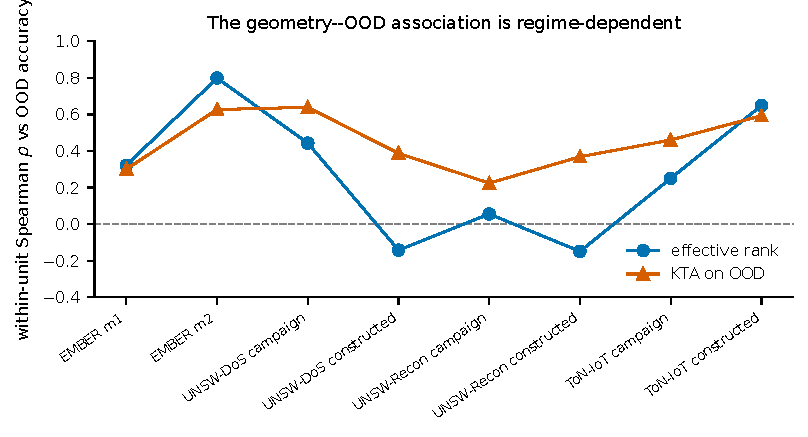
\includegraphics[width=0.72\textwidth]{fig_v4_mechanism.pdf}
\caption{The geometry--OOD association is regime-dependent. Median within-unit Spearman correlation between each geometry descriptor and OOD balanced accuracy, per scenario-group (SVC). Effective rank orders accuracy strongly in some regimes (EMBER $m2$, ToN-IoT $m2$) and weakly or negatively in others (the UNSW constructed-shift scenarios); OOD alignment is more consistently positive but never uniform. No single descriptor governs all regimes.}
\label{fig:mechanism}
\end{figure*}

\paragraph{The geometry--OOD link is a regime-dependent association, not a law.}
Two descriptors of the training and OOD Gram matrices carry information about which kernels generalize: the effective rank of the training kernel and the centered kernel-target alignment on the OOD split. But their association with OOD accuracy is regime-dependent, not a single mechanism. Within scenario-groups (Figure~\ref{fig:mechanism} and Supplementary Table~3), the median Spearman correlation between effective rank and OOD accuracy ranges from $+0.80$ (EMBER $m2$) down to $-0.15$ (UNSW-NB15 reconnaissance under the constructed shift); partial correlations that control for family label and length scale track the raw values closely. OOD alignment is more consistently positive ($+0.22$ to $+0.64$) but likewise varies by regime. A geometry model fit on three datasets and used to rank the held-out dataset's kernels achieves only Spearman $0.23$--$0.40$. We therefore describe a genuine but partial association, not a causal mechanism or deployable predictor.

\subsection{Finite-shot estimation: the geometry is a statevector idealization}
\label{sec:res_shots}

All quantum kernels above are computed by exact statevector simulation, which is the right idealization for a geometry study but not what a device would return. To probe how the picture degrades away from that idealization we apply a \emph{finite-shot fidelity-estimation perturbation model}: each fidelity entry is replaced by a binomial estimate from $s$ shots, train blocks are symmetrized, unit-diagonal, clipped to $[0,1]$, and projected to the positive-semidefinite cone (Section~\ref{sec:methods}). This is not a hardware simulation---no device noise, mitigation, or transpilation is modelled---but it isolates the statistical cost of estimating a fidelity from finite measurements. Table~\ref{tab:shots} reports the effect on the $q1000$ subset. OOD alignment and OOD accuracy are robust: median $\mathrm{KTA}_{\mathrm{OOD}}$ deviates by at most $0.0004$ from the exact value even at $128$ shots, and OOD balanced accuracy by $0.018$--$0.033$. Effective rank is not: finite sampling inflates it by a median factor of $2.1$ at $128$ shots, falling to $1.15$ only at $8192$ shots, because sampling noise adds spurious spectral mass. The within-family configuration selected by ID-validation changes identity under perturbation (agreement $7$--$21\%$), but the accuracy cost of that instability is negligible (mean regret $\le0.003$), so the flatness of the family optimum---already visible in the exact results---persists. The practical reading: the alignment description we can measure transfers to finite shots, but the effective-rank description, and any story that leans on it, is a statevector-exact quantity that would need many shots to reproduce.

% Table generated by scripts/reporting/make_v4_tables.py from results/v4/shots/
\begin{table}[t]
\centering
\caption{Finite-shot fidelity-estimation perturbation (EMBER+network $q1000$ subset, SVC). ``OOD acc.\ dev.'' is the median absolute deviation of OOD balanced accuracy from the statevector-exact value; ``KTA dev.'' the same for OOD alignment; ``rank ratio'' the median ratio of perturbed to exact effective rank; ``sel.\ agree'' the fraction of runs whose ID-validation-selected configuration is unchanged; ``regret'' the mean OOD accuracy lost by deploying the perturbed selection.}
\label{tab:shots}
\footnotesize
\setlength{\tabcolsep}{5pt}
\begin{tabular}{@{}cccccc@{}}
\toprule
Shots & OOD acc.\ dev. & KTA dev. & rank ratio & sel.\ agree & regret \\
\midrule
128 & 0.0327 & 0.0004 & 2.12 & 7\% & $+0.0007$ \\
512 & 0.0273 & 0.0001 & 1.56 & 10\% & $+0.0017$ \\
2048 & 0.0240 & 0.0001 & 1.29 & 19\% & $-0.0025$ \\
8192 & 0.0181 & 0.0000 & 1.15 & 21\% & $-0.0001$ \\
\bottomrule
\end{tabular}
\end{table}

\subsection{Predictive uncertainty under shift}
\label{sec:res_uncertainty}

The Laplace GP probabilities provide a secondary uncertainty check (Supplementary Figure~1). For the honestly selected candidate, predictive entropy rises from ID to OOD for both families in every scenario-group, while expected calibration error changes moderately and comparably. Because neither family has an accuracy advantage, the fidelity kernels show no calibration benefit unavailable to classical kernels. We do not interpret rising entropy alone as evidence of calibration.

\section{Discussion}
\label{sec:discussion}

\subsection{What is, and is not, a quantum advantage here}

The study's central interpretive move is to replace the question ``do quantum kernels beat classical kernels under shift?'' with ``which properties of a kernel are associated with its behaviour under shift, and does either family have exclusive access to them?''. Read through that lens, the results are clear and negative. The apparent advantage over linear and RBF baselines does not survive the combined correction of oracle selection, fixed regularization, and unequal candidate families. It does not reappear against the equal-budget extended family or at matched effective rank. The geometry descriptors carry information as regime-dependent associations rather than a governing law, and they are shared: a well-tuned heavy-tailed classical kernel occupies the same observed geometric regime as the fidelity maps. On present evidence there is no robust out-of-distribution advantage for fidelity kernels in the low-qubit settings studied, and the only residual---a modest in-distribution separability edge under the probabilistic classifier---is small, classifier-dependent, and itself shrinks under no-OOD-label selection.

From the perspective of the distribution-shift literature, this reinforces a general lesson: conclusions about robustness are only as credible as the protocol used to obtain them \cite{quinonero-candela2008datasetshift,gulrajani2021domainbed,koh2021wilds,yao2022wildtime}. Our results add a QML-specific corollary. The strength of the classical baseline, whether its regularization is tuned, whether model selection may consult the target labels, and the size of each family's candidate budget are not implementation details: each can move the quantum-versus-classical verdict, and together they turn an apparent $+0.037$ advantage into a null. A demonstration that fixes any of them in the quantum family's favour, reported alone, would mislead---and much of the optimistic quantum-kernel literature fixes several at once.

\subsection{The ID--OOD dissociation is informative}

In-distribution separability is the one axis on which the fidelity kernels retain any edge, and even it must be stated carefully. Under the oracle that selects and evaluates on the same in-distribution split, the quantum family separates the classes slightly better than linear+RBF in every EMBER setting; but under honest selection---choosing on a validation split and reporting on a disjoint test split---the edge falls to $+0.003$ under SVC (mixed in sign across groups) and $+0.012$ under the probabilistic classifier, and it does not translate into any out-of-distribution benefit. This ID--OOD dissociation is real but modest, and it cuts against, not for, an operational recommendation: a family that is marginally more separable in-distribution yet no more robust under shift offers nothing to a deployment whose whole difficulty is the shift. The pattern is consistent with the ``accuracy on the line'' literature \cite{miller2021accuracy}, in which ID and OOD accuracy usually move together; here they decouple weakly, and geometry---shared by both families---rather than quantumness marks the axis along which they do.

\subsection{The mechanism in context}

The geometry association connects several strands of literature. That length scale is decisive for kernel behaviour is known for both families \cite{shaydulin2022bandwidth,canatar2023bandwidth}; our contribution is the comparative consequence---once length scale is tuned symmetrically and regularization is tuned at all, the classical family reaches the same geometric regime, so asymmetric tuning does not merely bias quantum-versus-classical comparisons, it manufactures the apparent advantage. The geometric difference of Huang et al.\ \cite{huang2021powerofdata} does not predict which family wins a scenario, consistent with its definition as a bound on the \emph{potential} for a separation rather than its sign; a large geometric difference is compatible with equal or worse OOD accuracy, as we observe. That effective rank and OOD alignment are associated with performance is a statement about kernels in general, not about quantum kernels---which is precisely why the fidelity maps hold no privileged position: they are one costly route into a geometric regime that a short-length-scale classical kernel reaches directly.

The high-rank finding must also be reconciled with two spectral results that superficially point the other way. K\"ubler et al.\ argue that quantum kernels generalize in-distribution only when the relevant spectral mass is concentrated in few components \cite{kubler2021inductivebias}, and Thanasilp et al.\ show that fidelity kernels concentrate exponentially---toward effectively rank-one, uninformative Gram matrices---as qubit counts grow \cite{thanasilp2024concentration}. There is no contradiction, but there is a genuine tension that our results locate precisely. Both results concern the asymptotic or i.i.d.\ regime; our effective ranks (roughly $10$--$150$ on training sets of $10^3$--$4\times10^3$ samples at $4$--$12$ qubits) sit far below the concentration regime, so no contradiction arises. Our finite-shot analysis, however, adds an empirical caveat these theoretical results anticipate: effective rank measured from finitely estimated fidelities inflates substantially (Section~\ref{sec:res_shots}), so the exact effective ranks we report are a statevector idealization, and any account that leans on effective rank as the operative quantity would need many shots to reproduce even at the modest qubit counts studied here.

We emphasize what the geometry analysis does not deliver. It is a post-hoc association, not a deployable selection rule: choosing a configuration by training-set geometry alone does not reliably identify the better kernel, and OOD alignment requires OOD labels. Because the two families are statistically indistinguishable under honest selection, the more useful open problem is no longer ``which family wins'' but whether any label-free, train-only signal can select a robust kernel at all---a question that concerns classical and quantum kernels equally.

\subsection{Implications for security machine learning practice}

From a practical perspective, the paper suggests three takeaways for security ML. The first is substantive: on the evidence here, fidelity-based quantum kernels do not offer a robustness advantage under distribution shift over well-tuned classical kernels, while their pairwise overlap estimation introduces circuit and shot costs absent from direct evaluation of the classical baselines. A median-heuristic Laplacian kernel, especially one with a shortened length scale and its regularization tuned, is a strong and inexpensive robustness baseline, and it matches the fidelity maps under no-OOD-label selection on both modalities. Practitioners weighing a quantum-kernel pipeline for OOD-sensitive security detection should, on this evidence, prefer a tuned classical kernel unless a specific regime demonstrably favours the quantum construction after the same controls.

The second is methodological. Independently of the preferred kernel family, the protocol used here provides a reusable blueprint for robust evaluation in security settings:
\begin{enumerate}
    \item keep the classifier and preprocessing fixed, and swap only the kernel;
    \item define explicit OOD splits tied to interpretable shift mechanisms, including at least one non-constructed shift mechanism where the data permit;
    \item give every family the same freedom---the same candidate budget, symmetric length-scale tuning, and per-configuration regularization tuned on training data alone;
    \item select the deployed configuration without out-of-distribution labels, and keep an in-distribution test split disjoint from the validation split used for selection;
    \item repeat the pipeline, report variability as conditional intervals, and treat correlated benchmarks as fixed case studies rather than pooling them into a single population $p$-value.
\end{enumerate}
Security ML frequently suffers from comparisons in which model class, tuning effort, and evaluation conditions change simultaneously; the way the verdict of Sections~\ref{sec:res_baselines}--\ref{sec:res_honest} moves from a large apparent advantage to a null as the protocol is made fair is a concrete demonstration of how much the conclusion depends on getting this right.

The third concerns diagnostics: the geometry descriptors are cheap to compute from Gram matrices that the pipeline already builds, and the alignment-survival analysis can be run post hoc on any deployed kernel system with a labeled drift sample. Practitioners should nonetheless resist reading these results as a blanket recommendation to replace classical kernels; the responsible recommendation is to test the candidate families under the expected shift regime, using exactly the kind of protocol described here.

\subsection{Limitations and threats to validity}

Several limitations define the scope of our conclusions.

\paragraph{Shift operationalization.}
Our OOD splits cover three reproducible mechanisms---within-class sparsity-tail extremes, train-geometry-tail extremes, and a held-out attack-campaign shift on network traffic (an unseen attack campaign plus a capture-partition change, not a timestamped temporal split)---but not the full space of real-world drift processes. Explicit temporal splits on timestamped malware, family-based drift, and adversarially induced shift remain outside the study's scope, and our conclusions should be re-tested under them rather than assumed.

\paragraph{Kernel and encoding coverage.}
The classical family now spans seven kernels plus a bandwidth sweep, and both families receive symmetric tuning freedom, but neither candidate set is exhaustive: the quantum side is restricted to four commonly used fidelity feature maps at low qubit counts, and trained or task-adapted encodings, projected kernels, and deeper maps are not evaluated. The mechanism gives a concrete prediction for such extensions---what should matter is their Gram-matrix geometry, not their provenance---which future work can falsify. At substantially larger qubit counts, exponential kernel concentration \cite{thanasilp2024concentration} would erode the alignment-preserving rank the mechanism rewards, so our conclusions should not be extrapolated beyond the low-qubit regime studied here.

\paragraph{Selection over candidate sets.}
P1$'$ (ID-validation selection), P2 (cross-realization OOD-supervised selection), and P3 (same-test OOD oracle) are selection procedures over finite candidate sets. The primary comparison matches candidate budgets, and the full-pool and budget curves provide sensitivities, but residual dependence on candidate definitions and search granularity remains. Fully nested selection over additional independent benchmark pools would strengthen the analysis further.

\paragraph{Simulation, not hardware.}
All quantum kernels are computed by exact statevector simulation. The study therefore characterizes the geometry of fidelity kernels, not the behavior of noisy devices: finite sampling of kernel entries, hardware noise, and error mitigation would all perturb the Gram matrices \cite{wang2021nisq}, and exponential concentration implies that with polynomially many shots the very spectral richness our mechanism rewards becomes expensive to resolve at larger scales \cite{thanasilp2024concentration}; the effect of either on alignment survival is unknown and worth measuring. We make no claim about hardware feasibility, resource advantage, or quantum speedup---the only rigorously established quantum-classical learning separation concerns a specifically constructed problem, not natural data \cite{liu2021rigorous}. At the dimensions studied, the fidelity kernels are also classically simulable \cite{schreiber2023surrogates,jerbi2024shadows}, which is precisely what makes them available as practical kernel constructions today.

\paragraph{Dataset scope and feature caveats.}
Four benchmark scenarios across two modalities is a substantial widening relative to single-dataset studies, but security is broader still: dynamic malware analysis, encrypted traffic, and non-security modalities remain untested. Within the network scenarios, the feature sets inherited from the public benchmarks retain port numbers and protocol indicators, which are legitimate but known shortcut-prone features in NIDS benchmarks \cite{engelen2021troubleshooting}; because every kernel receives identical features, this affects absolute accuracies, not the family comparisons. Finally, the mechanism's effective-rank component is itself regime-dependent (strong on EMBER and ToN-IoT, weak on UNSW-Reconnaissance), a gradation we report rather than smooth over.

\subsection{Conservative interpretation}

In light of these limitations, the appropriate interpretation of the paper is deliberately conservative. We do not claim universal superiority, complexity-theoretic quantum advantage, or hardware relevance---nor do we claim to have refuted quantum kernels in general. We claim three narrower things, supported by conditional effect estimates rather than a population $p$-value: that the apparent out-of-distribution advantage of fidelity kernels over customary baselines disappears when same-test oracle selection and untuned regularization are removed; that under equal candidate budgets and no-OOD-label selection no robust family-level advantage remains against either the customary or the extended classical reference, across eight fixed scenario-groups and two classifiers; and that the geometric descriptors associated with out-of-distribution behaviour occur in both families and do not identify kernel provenance as the source of robustness. This view is consistent with recent calls for careful benchmarking in QML \cite{bowles2024betterthanclassical,schnabel2025scrutiny,kakavand2026benchmarking} and is more informative than either an unqualified advantage claim or an unqualified dismissal: it identifies the evaluation choices that generate the optimistic result and shows how the conclusion changes when they are controlled.


\subsection{Conclusion}
\label{sec:conclusion}

This paper asked why kernel families behave differently under distribution shift, using the quantum-versus-classical comparison as both motivation and stress test. A controlled kernel-swap protocol---classifier, preprocessing, splits, selection logic, and tuning freedom held fixed while only the kernel varies---was instantiated on four security scenarios spanning two modalities and three shift mechanisms, two classifier families including a probabilistic one, and 72 principal settings with fifteen pipeline realizations. Effects are reported as fixed-case summaries with conditional pipeline-realization intervals, not as population significance tests.

The empirical arc has three movements. Under same-test oracle selection and fixed regularization, fidelity-based quantum kernels appear to beat the customary linear and RBF baselines under shift. That result does not survive the controlled comparison: once each configuration is tuned on training data, selection uses no OOD labels, and both extended families search an equal budget of kernel geometries, the dataset-equal-weighted OOD difference is $-0.005$ under the primary SVC analysis and $-0.002$ under the GP classifier. The primary comparison is classical-favoured or tied in seven of eight scenario-groups. At matched effective rank the classical kernels are at least as accurate everywhere. Effective rank and OOD alignment are associated with performance in a regime-dependent way, are shared by both families, and, a finite-shot analysis shows, do not transfer unchanged from exact statevectors to finite measurement.

The contribution is therefore threefold. Empirically, the study provides a controlled, variability-aware comparison of quantum and classical kernels under shift whose central finding is a clean negative obtained under fair conditions: no robust family-level advantage survives budget matching, regularization tuning, and honest selection. Methodologically, it isolates the specific evaluation choices---oracle selection, fixed regularization, mismatched budgets, and pooled significance testing over correlated settings---that manufacture apparent quantum-kernel advantages, and it leaves behind a reproducible protocol that removes each. Analytically, it shows that the geometric quantities often invoked to explain such advantages describe both families equally and do not transfer unchanged to finite-shot estimation.

The most useful open problem this leaves is not ``which family wins'' but whether any label-free, train-only signal can select a robust kernel under shift at all; the security community's label-free drift detectors \cite{yang2021cade} and the theory of task--model alignment \cite{bordelon2020spectrum,canatar2021taskmodel,ma2023covariate} are natural starting points. It is a question about kernels in general, and answering it would benefit classical and quantum methods alike---which is, in the end, the point: the productive question is not whether one family dominates, but which similarity geometry aligns with the shift regime one actually faces, and how to find it without peeking.

\section{Methods}
\label{sec:methods}

\subsection{Problem setting}

We study binary security classification---malware versus benign software, and attack versus benign traffic---under distribution shift. Let $D_{\mathrm{ID}}$ denote the in-distribution data-generating process and $D_{\mathrm{OOD}}$ an out-of-distribution process induced by a constructed stress test or a held-out attack campaign. Given training data $T\sim D_{\mathrm{ID}}$, we evaluate on an ID test set $S_{\mathrm{ID}}$ and an OOD test set $S_{\mathrm{OOD}}$.

To isolate the kernel, classifier, preprocessing, optimization protocol, and split design are fixed. Classical and quantum Gram matrices are therefore consumed by the same downstream learner on the same samples.

\subsection{Datasets and split construction}

The four scenarios span static malware (EMBER) \cite{anderson2018ember} and network flows: UNSW-NB15 DoS, UNSW-NB15 Reconnaissance \cite{moustafa2015unsw}, and ToN-IoT Scanning \cite{alsaedi2020toniot}. Every setting has shared $T$, $S_{\mathrm{ID}}$, and $S_{\mathrm{OOD}}$ samples with identical class balance across kernel families.

EMBER uses two label-conditional tail stress tests. The $m1$ split holds out within-class extremes of feature-block sparsity; $m2$ holds out within-class extremes of distance to train-fitted class centroids. Network scenarios use an analogous train-centroid construction and a held-out attack-campaign regime. In the latter, training and ID pools contain benign traffic plus non-target attacks, whereas OOD contains benign traffic plus the target campaign; UNSW pools additionally differ in capture partition. These are reproducible stress tests, not timestamped temporal splits or certified covariate shifts. Exact algorithms, feature exclusions, leakage checks, and pool definitions are in the Supplementary Note ``Dataset and shift construction.''

\subsection{Controlled kernel-swap protocol}

Figure~\ref{fig:protocol} summarizes the controlled pipeline. Both SVC and a binary Gaussian-process classifier with a logistic-link Laplace approximation consume unit-diagonal precomputed Gram matrices \cite{cortes1995svm,rasmussen2006gpml}. Comparisons are always within a classifier. The GP classifier supplies approximate probabilities for uncertainty diagnostics; no post-hoc calibration is applied.

Training-fitted MaxAbs scaling and TruncatedSVD produce shared representations at $d\in\{4,6,8,10,12\}$. Quantum inputs are then mapped linearly to $[0,\pi]$. Dimension is an explicit candidate axis.

\subsection{Kernel families}

The customary classical reference contains linear and RBF kernels. The extended reference adds degree-2 and degree-3 polynomial, Laplacian, and Mat\'ern-$3/2$ and $5/2$ kernels. RBF, Laplacian, and Mat\'ern bandwidths sweep factors $\{0.1,0.3,1,3,10\}$ around training-only scale or median-distance heuristics. The quantum family uses fidelity
\[
K_Q(x,x')=|\langle\phi_Q(x),\phi_Q(x')\rangle|^2
\]
for two ZZ depths, PauliXZ, and Z feature maps \cite{havlicek2019quantumenhanced,schuld2019featurehilbert}. Every map sweeps angle scales $\{0.5,1,2\}$. Classical bandwidth and quantum angle-scale freedom are symmetric in purpose \cite{shaydulin2022bandwidth,canatar2023bandwidth}. Exact formulas and grids appear in the Supplementary Note ``Controlled kernel-swap protocol.''

\subsection{Selection, candidate budgets, and inference}

For each geometry, SVC regularization $C\in\{0.01,0.1,1,10,100\}$ is selected by five-fold stratified cross-validation on the training Gram matrix. The primary P1$'$ protocol divides the ID holdout into disjoint validation and test halves. Within each family, the candidate with the highest ID-validation balanced accuracy is deployed on ID-test and OOD-test; OOD labels never enter this choice. Same-test OOD-oracle and cross-realization OOD-supervised protocols are descriptive sensitivities.

Best-of-family selection favours a larger pool. The primary extended-family endpoint therefore uses 60 candidates per family where coverage is complete and 20 where it is reduced, generated by 5,000 classical-pool subsamples under three schemes. The full 115-candidate classical pool is secondary.

Every configuration has fifteen pipeline realizations (five split seeds by three model seeds). Two EMBER and six network scenario-groups are crossed with three master seeds and $(n_{\mathrm{train}},n_{\mathrm{ID}},n_{\mathrm{OOD}})$ regimes $(1000,500,500)$, $(2000,1000,1000)$, and $(4000,1800,1800)$. Because scenario-groups share source pools and are not exchangeable, they are fixed case studies. Per group we average over the five split-seed clusters and report a conditional interval; across groups we use dataset-equal means and leave-one-dataset-out ranges. We attach no population $p$-value to eight fixed, correlated cases. The complete grid is in Supplementary Table~1 and resampling details in the Supplementary Note ``Controlled kernel-swap protocol.''

\subsection{Metrics and geometry analysis}

OOD balanced accuracy is primary. Family effects are quantum minus classical after selection. ID balanced accuracy and ID-to-OOD degradation are secondary. For the GP classifier we also record log loss, Brier score, 15-bin expected calibration error \cite{guo2017calibration}, and predictive entropy.

From the classifier Gram matrices we compute effective rank \cite{roy2007effective}, centered kernel-target alignment \cite{cristianini2001kta,cortes2012centeredalignment}, entry concentration, cross-split similarity, and regularized geometric difference \cite{huang2021powerofdata}. We relate geometry to OOD accuracy within scenario-groups, use partial association to control family and length scale, test portability by leaving one dataset out, and pair quantum candidates with nearest-effective-rank classical candidates within run and dimension. These analyses are associational. Formulas and diagnostic definitions appear in the Supplementary Note ``Metrics and geometry descriptors.''

\subsection{Finite-shot perturbation}

Exact fidelity entries are replaced by binomial estimates at $s\in\{128,512,2048,8192\}$ shots. Training blocks are symmetrized, clipped, set to unit diagonal, and projected to the positive-semidefinite cone. The model isolates sampling error, not device noise. Projection diagnostics and interpretation are in the Supplementary Note ``Finite-shot fidelity-estimation model.''

\subsection{Use of generative AI}

OpenAI Codex was used during manuscript revision to assist with language editing, code inspection, and consistency checking. The authors reviewed and take responsibility for all analyses, claims, citations, and text; the system is not an author.

\backmatter

\section*{Declarations}

\bmhead{Data availability}
This study uses the public EMBER \cite{anderson2018ember}, UNSW-NB15 \cite{moustafa2015unsw}, and ToN-IoT \cite{alsaedi2020toniot} benchmarks, which remain subject to their original access conditions. Derived split definitions, shift constructions, experiment manifests, aggregated results, and summary tables are available in the Zenodo repository at \url{https://doi.org/10.5281/zenodo.19147649}. Before submission, this DOI will be verified against the exact archived release used to build the manuscript.

\bmhead{Code availability}
Code for constructing the splits, running the kernel experiments, reproducing the confirmatory analysis, and regenerating every table and figure is available at \url{https://github.com/roberto-fernandez-barrios/kernel_shift_framework} and in the versioned Zenodo archive above. The platform-independent Python 3.12 environment is pinned in \texttt{environment.lock.yml}; the code is released under BSD-3-Clause with no restriction on non-academic use.

\bmhead{Competing interests}
The authors declare that they have no competing interests.

\bmhead{Funding}
The authors received no specific funding for the submitted work.

\bmhead{Authors' contributions}
RFB: conceptualization, methodology, software, data curation, formal analysis, visualization, investigation, writing---original draft, writing---review and editing. IPL: supervision, validation, writing---review and editing. AGS: validation, project administration, writing---review and editing. PGB: supervision, resources, writing---review and editing. All authors read and approved the final manuscript.

\bmhead{Acknowledgements}
Not applicable.



%%===========================================================================================%%
%% If you are submitting to one of the Nature Portfolio journals, using the eJP submission   %%
%% system, please include the references within the manuscript file itself. You may do this  %%
%% by copying the reference list from your .bbl file, paste it into the main manuscript .tex %%
%% file, and delete the associated \verb+\bibliography+ commands.                            %%
%%===========================================================================================%%

\bibliography{sn-bibliography}% common bib file
%% if required, the content of .bbl file can be included here once bbl is generated
%%\input sn-article.bbl

\end{document}
